\documentclass[a4paper]{article}

% formatting
\usepackage[utf8]{inputenc} % allow utf-8 input
\usepackage[T1]{fontenc} % use 8-bit T1 fonts  (allows for direct use of ö,ü,etc.)

% math typesetting
\usepackage{amsmath}
\usepackage{amssymb}
\usepackage{amsfonts}

% maths definitions, theorems, etc.
\usepackage{amsthm}

% color
\usepackage{color}
\usepackage{xcolor}

% layout
\usepackage{layout}
\usepackage{lipsum}

% cross-referencing and hyperlinks
\usepackage{hyperref}
\usepackage{url}
\usepackage{doi}

% figures
\usepackage{graphicx}
\usepackage{subfig}
\usepackage{wrapfig}

% tables
\usepackage{booktabs}
\usepackage{multirow}
\usepackage{caption} 
\usepackage{float}

% enumeration
\usepackage{enumitem}

% embedding pages
\usepackage{pdfpages}

% multi-line comments
\usepackage{comment}

% landscape orientation
\usepackage{rotating}
\usepackage{pdflscape}

% Gantt charts
\usepackage{pgfgantt}

% footnotes
\usepackage{footnote}

% code
\usepackage{listings}

% matrices and tables
\usepackage{nicematrix}
\usepackage{varwidth}
% \usepackage{tabularx} do not load package tabularx, instead use package nicematrix

% document structure
\setcounter{secnumdepth}{5} % enable numbered sub-sub-sections etc.

% custom header size
\usepackage{titlesec}

% customized references (make "Figure 1" a link, not just "1")
\usepackage[capitalise, nameinlink]{cleveref}

% customized frames around text etc.
\usepackage{mdframed}

% tikz
\usepackage{tikz}

% calligraphy
\usepackage{calligra}

% chemical formulas
\usepackage{chemformula}
% column layout
\usepackage{multicol}
\setlength{\columnsep}{0.75cm}

% paragraphs
\usepackage[skip=0.5\baselineskip]{parskip}

% geometry
\usepackage[
    margin = 3cm,
    top = 3cm,
    bottom = 3cm
]{geometry}

% header size
\usepackage{titlesec}
\titleformat*{\section}{\large\bfseries}
\titleformat*{\subsection}{\normalsize\bfseries}
\titleformat*{\subsubsection}{\normalsize\bfseries}
\titleformat*{\paragraph}{\normalsize\bfseries}
\titleformat*{\subparagraph}{\normalsize\bfseries}

% custom headers
\usepackage{fancyhdr}
\pagestyle{fancy}
\fancyhead{}
\fancyfoot{}
\renewcommand{\headrulewidth}{0.4pt} % Keep header line
\setlength{\headheight}{15pt}
\setlength{\headsep}{10pt}
\renewcommand{\sectionmark}[1]{}
\renewcommand{\subsectionmark}[1]{}

\usepackage[
    backend=biber,
    style=ieee
]{biblatex}
\addbibresource{references.bib}
% show DOI URL (https://doi.org/XXX.XXXXX.XXXX), instead of publisher URL (https://springer.com/XXXX)
% cf. https://tex.stackexchange.com/a/616241
\DeclareSourcemap{
  \maps[datatype = bibtex]{
    \map{
      \step[notfield = keywords, final]
      \step[fieldsource = doi, final]
      \step[fieldset = url, null]
    }
    \map{
      \step[fieldsource = keywords, notmatch = \regexp{\bprimary\b}, final]
      \step[fieldsource = doi, final]
      \step[fieldset = url, null]
    }
  }
}
\AtEveryBibitem{
    \clearfield{urlyear}
    \clearfield{urlmonth}
}

\usepackage{tikz}

% https://tex.stackexchange.com/a/294990
\newcommand{\ExternalLink}{
    \tikz[x=1.2ex, y=1.2ex, baseline=-0.05ex]{
        \begin{scope}[x=1ex, y=1ex]
            \clip (-0.1,-0.1) 
                --++ (-0, 1.2) 
                --++ (0.6, 0) 
                --++ (0, -0.6) 
                --++ (0.6, 0) 
                --++ (0, -1);
            \path[draw, 
                line width = 0.5, 
                rounded corners=0.5] 
                (0,0) rectangle (1,1);
        \end{scope}
        \path[draw, line width = 0.5] (0.5, 0.5) 
            -- (1, 1);
        \path[draw, line width = 0.5] (0.6, 1) 
            -- (1, 1) -- (1, 0.6);
        }
    }

\renewcommand{\contentsname}{\centering Contents} % https://tex.stackexchange.com/a/308207
\usepackage[titles, subfigure]{tocloft} % https://tex.stackexchange.com/a/336618
\renewcommand{\cftsecleader}{\cftdotfill{\cftdotsep}} % https://tex.stackexchange.com/a/271942

%%%%%%%%%%%%%%%%%%%%%%%%%%%%%%%%%%%%%%%%%%%%%%%%%%%%%%%%%%%%%%%%%%%%%

% document metadata
\title{Proposal for a Summer Academy \protect\\ on Biophilic Design in Architecture}
\author{Michael P. Weinold$^1$, Philippe Schultheiss$^1$, Mark C. Ballandies$^2$}
\date{
    $^1$Schweizerische Studienstiftung \\
    $^2$Stiftung der Deutschen Wirtschaft \\[3mm]
    October 2023
}

%%%%%%%%%%%%%%%%%%%%%%%%%%%%%%%%%%%%%%%%%%%%%%%%%%%%%%%%%%%%%%%%%%%%%

\begin{document}

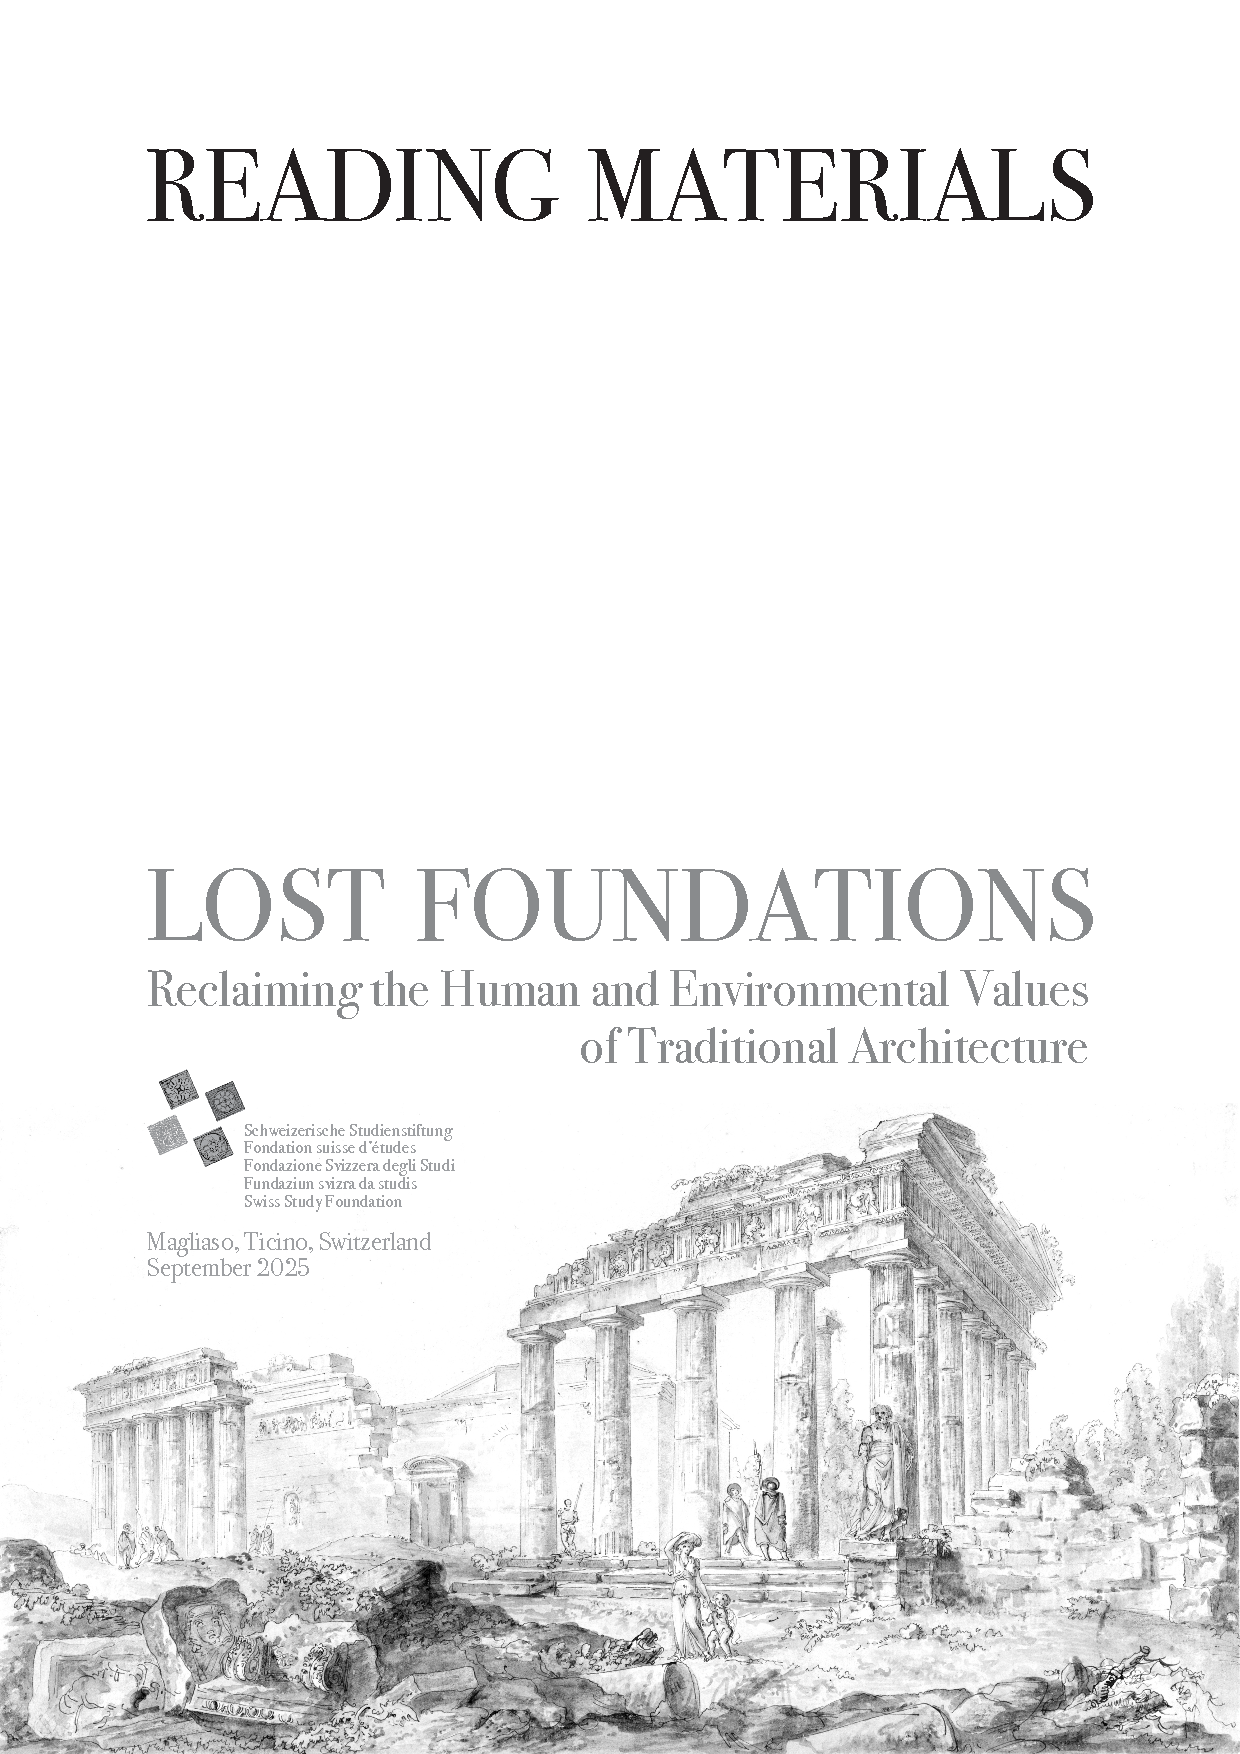
\includepdf[]{figures/cover.pdf}

\maketitle

\section*{\centering Authors}
\vspace{-10mm}

\begin{tikzpicture}[remember picture, overlay]
    \node[xshift=-10.3cm, yshift=+0.75cm, font=\small] at (current page.south east) {\textit{two dandelions of the genus Taraxacum, most often associated with the archetype of flowers springing from concrete}};
\end{tikzpicture}

\textbf{\textit{Michael P. Weinold}} (born 1995 in Innsbruck, Austria) is a doctoral researcher at ETH Zurich and the Paul Scherrer Institute. His background is in engineering physics, with degrees from Vienna University of Technology and ETH Zurich. His current research is focused on accelerating innovation in novel clean-energy technologies. He builds mathematical models and open-source software to better help decision makers assess the environmental impact of different techno-economic scenarios for decarbonizing the economy. Since 2023, he is a guest lecturer at the Department of Mechanical Engineering of ETH Zurich. His interest in aesthetics in the built environment was sparked during his research at the University of Cambridge, where he was introduced to the legacy of the late British philosopher Sir Roger Scruton. Since that time, he has been most interested in how new neuro-scientific insights can enable citizen movements to positively shape public spaces.

\textbf{\textit{Philippe Schultheiss}} (born 1984 in Basel, Switzerland) is a consultant and soon-to-be pastor in the Swiss Reformed Church. He holds undergraduate degrees in Business \& Economics from the university of Basel as well as a master's degree in Medieval Philosophy from the university of Freiburg i.Ue. He is now an alumnus of the Swiss Study Foundation, where he is still active as a member of the Assessment Jury as well as a frequent host of events. He has been interested in politics, especially the areas of environmental and urban planning, since his days at the cantonal school at Schaffhausen. He went on to co-found the Green-Liberal Party in his home canton and remained involved in local politics after his relocation to Zurich, where, in 2020, he was elected president of the Parliament of the Reformed Church Zurich. This community of more than 70'000 members administers dozens of church buildings. Hence his motivation to contribute to a prospective and socially beneficial real estate strategy.

\textbf{\textit{Mark C. Ballandies}} (born 1991 in Burgwedel, Germany) is a postdoctoral researcher in the Computational Social Science group at ETH Zurich, where he is exploring decentralised, bottom-up and community-owned solutions to complex societal challenges. In addition, he is involved in the startup WiHi that uses a decentralized network of stations to improve weather and climate predictions. He is the co-founder of DAOSuisse, a lecturer at the Vorarlberg University of Applied Sciences, an alumnus of the Foundation of German Business, president of education matters e.V. and initiator of the Smarte Dörfer association. In 2019, Mark discovered the beauty of old farmhouses and their effectiveness in combating environmental challenges when he began restoring a half-timbered house in his home village, using ecological, locally sourced and recyclable building materials such as wood, clay and hemp. He found that these farmhouses integrate values such as circularity, sustainability and locality into all aspects and details of their design and construction, resulting in unique, sustainable and liveable architecture. This discovery inspires him in his daily work, which he enjoys sharing with others.

\clearpage

\section*{\centering Administrative Information}

\begin{NiceTabularX}{\textwidth}{llX}
\textit{Author} & \textit{Email} & \textit{Phone} \\
\hline
Michael P. Weinold & \texttt{michael@weinold.ch} & \texttt{+41 75 500 70 70} \\
Philippe Schultheiss & \texttt{phschultheiss@protonmail.ch} & \texttt{+41 79 768 53 15} \\
Mark C. Ballandies & \texttt{bcmark@protonmail.com} & \texttt{+41 78 899 87 85}
\end{NiceTabularX}

\tableofcontents

\clearpage
\section{Abstract}
\label{sec:abstract}

We live in a time of unprecedented global construction activity. All major urban regions are experiencing strong growth, fuelled by the unabated population increase in some countries and increasing levels of migration in others. \\

The construction sector is now responsible for more than 40\% of annual global carbon emissions. Since the majority of construction-related emissions are hard to abate, this number is expected to grow for the foreseeable future. Despite the urgency of reducing carbon emissions, new buildings are often designed with a service life of around 50 years only. At the same time, a growing number of opinion polls point toward a deep-rooted dissatisfaction among the general population with the modernist style in which the majority of buildings is now designed. This is supported by a number of recent neuro-scientific experiments. \\

This disconnect between the taste of architects and the general public is by no means a novel phenomenon and has been widely caricatured, as illustrated in \cref{fig:loewy}. However, recent work by contemporary philosophers, including Sir Roger Scruton \textit{"Why Beauty Matters"} and Alain de Botton \textit{"Why is the Modern World So Ugly?"} have re-invigorated public debate. \\

Architects, from the founders of modernism to present day proponents of brutalist structures have repeatedly rejected calls for more traditional designs, instead aiming to "re-educate" the public through their designs. With architecture often likened to \textit{a gallery you can't walk out of}, citizen initiatives have formed, all asking the question: "How can we ensure our cities do not become mazes of concrete and glass? \\

In light of these bleak developments, cognitive scientists, citizen initiatives and a select group of architects and designers have pointed to \textit{biophilic design} as a tangible remedy to the featureless façades that have come to dominate real estate projects in recent decades. Building design inspired by nature, in both the aesthetic and the functional dimension, has the potential to significantly improve the wellbeing of citizens while reducing the environmental footprint of construction. \\

We propose to invite a group of speakers that, through their academic or professional work, are shaping the current conversation around architecture, beauty and nature. The participants of the academy will learn why architects came to believe that \textit{béton brut} was the material of the future, what the real environmental footprint of modern construction is, if and how we can ever hope to quantify the aesthetics of a building, how we can learn from nature to build better, how citizen action can help shape the (un-)built environment $\dots$ and so much more.

\clearpage
\section{Architecture History}

\subsection{Ornament and Crime (Adolf Loos)}

Delivered in a lecture on 21 January 1910 to the Vienna Akademischer Verband fur Literatur und Musik

Some words on Adolf Loos

\begin{figure}[h]
  \centering
  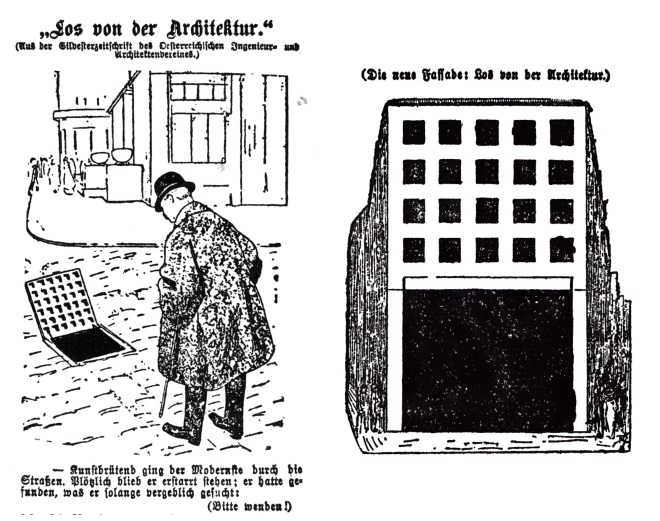
\includegraphics[width=0.7\textwidth]{./figures/caricature_loos.jpg}
  \caption{\textit{"Kunstbrütend ging der Modernste durch die Stassen. Plötzlich blieb er erstarrt stehen. Er hatte gefunden was er solange vergeblich gesucht: Die neue Fassade: Los von der Architektur!"}, contemporary caricature of Adolf Loos, published 1911 in the Viennese newspaper "Illustrirtes Wiener Extrablatt".}
  \label{fig:caricature_loos}
\end{figure}


In the womb the human embryo passes through all the development stages of the animal kingdom. At the moment of birth, human sensations are equal to those of a newborn dog. His childhood passes through all the transformations which correspond to the history of mankind. At the age of two, he sees like a Papuan, at four, like a Teuton, at six like Socrates, at eight like Voltaire. When he is eight years old, he becomes aware of violet, the colour which the eighteenth century had discovered, because before that the violet was blue and the purple snail red. Today the physicist points to colours in the sun’s spectrum which already bear a name, whose recognition, however, is reserved for the coming generation.

The child is amoral. To us the Papuan is also amoral. The Papuan slaughters his enemies and devours them. He is no criminal. If, however, the modern man slaughters and devours somebody, he is a criminal or a degenerate. The Papuan tattoos his skin, his boat, his oar, in short, everything that is within his reach. He is no criminal. The modern man who tattoos himself is a criminal or a degenerate. There are prisons where eighty percent of the inmates bear tattoos. Those who are tattooed but are not imprisoned are latent criminals or degenerate aristocrats. if a tattooed person dies at liberty, it is only that he died a few years before he committed a murder.

The urge to ornament one’s face, and everything in one’s reach, is the origin of fine art. It is the babble of painting. All art is erotic.

The first ornament that came into being, the cross, had an erotic origin. The first work of art, the first artistic action of the first artist daubing on the wall, was in order to rid himself of his natural excesses. A horizontal line: the reclining woman. A vertical line: the man who penetrates her. The man who created it felt the same urge as Beethoven, he experienced the same joy that Beethoven felt when he created the Ninth Symphony.
But the man of our time who daubs the walls with erotic symbols to satisfy an inner urge is a criminal or a degenerate. It is obvious that his urge overcomes man: such symptoms of degeneration most forcefully express themselves in public conveniences. One can measure the culture of a country by the degree to which its lavatory walls are daubed. With children it is a natural phenomenon: their first artistic expression is to scrawl on the walls erotic symbols. But what is natural to the Papuan and the child is a symptom of degeneration in the modern man. I have made the following observation and have announced it to the world: The evolution of culture is synonymous with the removal of ornament from objects of daily use. I had thought to introduce a new joy into the world: but it has not thanked me for it. Instead the idea was greeted with sadness and despondency. What cast the gloom was the thought that ornament could no longer be produced. What Are we alone, the people of the nineteenth century, are we no longer capable of doing what any Negro can do, or what people have been able to do before us?
Those objects without ornament, which mankind had created In earlier centuries, had been carelessly discarded and destroyed. We possess no carpenter’s benches of the Carolingian period: instead any rubbish which had even the smallest ornament was collected, cleaned and displayed in ostentatious palaces that were built for them, people walked about sadly amongst the display cabinets. Every period had its style: why was it that our period was the only one to be denied a style? By “style” was meant ornament. I said, “Weep not. Behold! What makes our period as important is that it is incapable of producing new ornament. We have outgrown ornament, we have struggled through to a state without ornament. Behold, the time is at hand, fulfilment awaits us. Soon the streets of the cities will glow like white wand Like Zion, the Holy City, the capital of heaven. It is then that fulfilment will have come.”

But there are still hobgoblins who will not allow it to happen. Humanity is still to groan under the slavery of ornament. Man had progressed enough for ornament to no longer produce erotic sensations in him, unlike the Papuans, a tattooed face did not increase the aesthetic value, but reduced it. Man had progressed far enough to find pleasure in purchasing a plain cigarette case, even if it cost the same as one that was ornamented. They were happy with their clothes and they were glad that they did not have to walk about in red velvet trousers with gold braids like monkeys at a fun fair. And I said: “Behold, Goethe’s death chamber is more magnificent than all the pomp of the Renaissance, and a plain piece of furniture is more beautiful than all the inlaid and carved museum pieces. Goethe’s language is more beautiful than all the ornaments of the shepherds of the Pegnitz.”

This was heard by the hobgoblins with displeasure. The state, whose duty it is to impede people in their cultural development, took over the question of development and re-adoption of ornament and made it its own. Woe betide the state, whose revolutions are brought about by its privy councillors!
Soon one was to see a buffet introduced into the Viennese Museum of Applied Arts, which was called “the prosper°us fish shoal,” them was even a cupboard, which was given the trade name “the cursed princess” or something similar, which referred to the ornament with which this unfortunate piece of furniture was covered. The Austrian state takes its task an seriously that it ensures that outdated footwear will not disappear from within the boundaries of the Austro-Hungarian Empire. The state forces every cultivated twenty-year-old man to wear outdated footwear for three years (after all, every state proceeds on the assumption that a poorly developed population is more easily governed). Well, the epidemic of ornament is recognised by the state and is subsidised with government money. I, however, consider that to be a regressive. I will not subscribe to the argument that ornament increases the pleasure of a life of a cultivated person, or the argument which covers itself with the words: “But if the ornament is beautiful!…” To me, and to all the cultivated people, ornament does not increase the pleasures of life. If I want to eat a piece of gingerbread I will choose one that is completely plain and not a piece which represents a baby in arms of a horserider, a piece which is covered over and over again with decoration. The man of the fifteenth century would not understand me. But modern people will. The supporter of ornament believes that the urge for simplicity is equivalent to self-denial. No, time professor from the College of Applied Arts, I am not denying myself! To me, it tastes better this way. The dishes of the past centuries which used decoration to make the peacocks, pheasants and lobsters appear more appetising produce the opposite effect on me. I look on such a culinary display with horror when I think of having to eat these stuffed animal corpses. I eat roast beef.

The immense damage and devastation which the revival of ornament has caused to aesthetic development could easily be overcome because nobody, not even the power of the state, can stop the evolution of humanity! It represents a crime against the national economy, and, as a result of it, human labour, money and material are mined. Time cannot compensate for this kind of damage.

The rate of cultural development is held back by those that cannot cope with the present. I live in the year 1908, but my neighbour lives approximately in the year Iwo, and one over there lives in the year 1880. It is a misfortune for any government, if the culture of its people is dominated by the past. The farmer from gals lives in the twelfth century, and on the occasion of the Jubilee Procession, tribes walked past which even during the period of mass migration were thought to be backward. Happy is the country which does not have such backward-looking inhabitants. Happy is America! Even here we have people in the cities who are survivors from the eighteenth century, and who are appalled by a painting with violent shadows, bemuse they cannot understand why the artist has used violet. To them, the pheasant which the cook has spent days preparing tastes better, and the cigarette case with Renaissance ornaments is more pleasing. And what Is happening in the countryside? Clothes and household utensils belong to previous centuries. The farmer is no Christian, he is still a heathen.

Those who measure everything by the past impede the cultural development of nations and of humanity itself. Ornament is not merely produced by criminals, it commits a crime itself by damaging national economy and therefore its cultural development. Two people living side by side who have the same needs, the same demands on life, and the same income, but belong to different cultures, perceive the national economy differently. The result is that the man of the twentieth century becomes richer and the man of the eighteenth century becomes poorer. I assume that both their lifestyles reflect their different attitudes. The man of the twentieth century can satisfy his needs with a much smaller capital and can, therefore, set aside savings. The vegetable which is appetising to him is simply boiled in water and has butter spread over it. To the other man it will only taste good if honey and nuts are added to it and it has been cooked by someone for hours. Decorated plates are expensive, while white crockery, which is pleasing to the modern individual, is cheap. Whilst one person saves money, the other becomes insolvent. This is what happens to entire nations. Woe betide the nation that remains behind in its cultural development. The English become richer and we become poorer…

In a highly productive nation ornament is no longer a natural product of its culture, and therefore represents backwardness or even a degenerative tendency. As a result, those who produce ornament are no longer given their due reward. We are aware of the conditions that exist in the wood carving and turning trades, the very low wages that are paid to the embroiderers and lace makers. The producer of ornament must work for twenty hours to obtain the same income of a modem labourer who works for eight hours. As a rule, ornament increases the price of the object. All the same there are occasions when an ornamented object is offered at half the price, despite the same material cost and production time, which works out to be three Pines longer as that of a plain unornamented object. The lack of ornament results in reduced working hours and an increased wage. The Chinese carver works sixteen hours, the American labourer works eight hours. If I pay as much for a plain box as I would for an un-ornamented one, then the difference is in working hours. And if there existed no ornament at all, a condition which might arise in millennia, man would only need to work four instead of eight hours, as the time spent on ornament represents half of today’s working day.
Ornament is wasted manpower and therefore wasted health. It has always been like this. But today it also means wasted material, and both mean wasted capital.

As ornament is no longer organically related to our culture, it is also no longer the expression of our culture. The ornament that is produced today bears no relation to us, or to any other humane the world at large. It has no potential for development. What happened to Otto Eckmann’s ornaments, and those of Van de Velde? The artist always stood at the centre of humanity, full of power and health. The modem producer of ornament is, however, left behind or a pathological phenomenon. He disowns his own products after only three years. Cultivated people find them instantaneously intolerable, others become conscious of their intolerability after many years. Where are Otto Eckmann’s products today? Where will Olbeich’s work be, ten years from now? Modern ornament has no parents and no offspring, it has no past and no future. Uncultivated people, to whom the significance of Our time is a sealed book, welcome it with joy and disown it after a short while.

Today, mankind Is healthier than ever before; only a few are ill. These few, however, tyrannise the worker, who is no healthy that he is incapable of inventing ornament. They force him to execute ornament which they have designed, in the most diverse materials.
The change in ornament implies a premature devaluation of labour. The worker’s rime, the unlined material is capital that has been wasted. I have made the statement. The form of the object should be bearable for as long as the object lasts physically. I would like to try to explain this: A suit will be changed more frequently than a valuable for coat. A lady’s evening dress, intended for one night only, will be changed more rapidly than a writing desk. Woe betide the writing desk that has robe changed as frequently as an evening dress, just because the style has become unbearable. Then the money that was spent on the writing desk will have been wasted.

This fact is well known to the Austrians who promote decoration and try to justify it by saying: “A consumer who owns furnishings which become unbearable to him, after only ten years, and who is therefore forced to buy furniture every ten years, is preferable so one who only buys an object for himself once the old one can no longer be used. Industry demands it. Millions of people are employed because of this rapid change.” This appears to be the secret of the Austrian national economy: how often does one hear the words uttered on the occasion of the outbreak of a fire: “Thank God: now there will be some work again.” I know a good remedy! Set a whole city on fire, net the entire Empire alight and everyone will wallow in money and wealth. Let an have furniture made which can be used for firewood after three years; lam have ironmongery which will have to be melted down after four years, as it is impossible to realise even a tenth of the original labour and material costs at the pawn-brokers, and we will become richer and richer.

The loss not only hits the consumer; it hits primarily the producer. Today, decorated objects, which, thanks to progress, have become separated from the realm of ornamentation, imply wasted labour and materials. Hall objects were to last as long in aesthetic terms as they did physically, the consumer could pay a price for them which would enable the labourer to earn more money and work shorter hours. I would gladly pay forty crowns for my boots even though I could obtain boots for ten crowns at another store. But in every trade which languishes under the tyranny of the ornamentalists, neither good our bad work is valued. Labour suffers because no one is prepared to pay for its true value.

Thank goodness that this is the case, because these ornamented objects are only bearable in the shabbiest execution. I recover from the news of a fire more rapidly if I hear that only worthless rubbish was burnt. I can be happy about the junk in the Künstlerhaus (the Municipal art gallery in Vienna), as I know that they pus on exhibitions in a few days which are pulled down in one. But the flinging of gold coins instead of pebbles, the lighting of a cigarette with a banknote, the pulverisation and drinking of a pearl appear unaesthetic.

Ornamented objects appear truly unaesthetic if they have been executed in the best material, with the highest degree of meticulous detail, and if they have required a long production dmc. I cannot plead innocence for having been the first to all for quality labour, but MK this kind of work.

The modern man who holds ornament sacred as the sign of artistic achievement of past epochs will immediately recognise the tortured, laboriously extracted and pathological nature of modern ornament. Ornament can no longer be borne by someone who exists at our level of culture. It is different for people and nations who have not reached this level.

I preach to the aristocrats, I mean the individuals who stand at the pinnacle of humanity and nevertheless have the deepest understanding for the motivations and privations of those who stand further below. The Kafir who weaves fabric according to a specific order which only appears when one unravels it, the Persian who ties his carpets, the Slovak farmer’s wife who embroiders her lace, the old lady who makes beautiful things with glass, beads and silk; all these he understands very well. The aristocrat lets them have their own way; he knows that they arc sacred hours in which they work. The revolutionary would come and say: “it is all nonsense.” As he would pull the old lady away from the roadside shrine and say to her: “There is no God.” But the atheist amongst she aristocrats lifts his hat as he walks past a church.

My shoes are covered all over with ornaments, which result from notches and holes: work which the cobbler carried out and which he was not paid for. I go to the cobbler and say to him “For a pair of shoes you are asking thirty crowns. I will pay you forty crowns.” By doing this I have made him happy and he will thank me for it by the work and materials which will not bear any relation in terms of quality to the extra amount. He is happy because rarely does fortune enter his house and he has been given work by a man who understands him, who appreciates his work and who does not doubt his honesty. He already imagines the finished pair in front of him. He knows where the best leather is to be found today, he knows which worker he will entrust with she shoes, and that they will display notches and hales, as many as there is space for on an elegant pair of shoes. And now I say: “But there is one condition which I have. The shoes must be completely smooth.” By that, I have plunged him from the height of happiness to the depths of Tartarus. He has less work to do, I have robbed him of all pleasures.

I preach to the aristocrats. I allow decoration on my own body, if it provides a source of pleasure for my fellow men. Then they are also my pleasures.1 suffer the ornament of the Kafir, that of the Persian, that of the Slovak farmer’s wife, the ornaments of my cobbler, because they all have no other means of expressing their full potential. We have our culture which has taken over from ornament. After a day’s trouble and pain, we go to hear Beethoven and Wagner. My cobbler cannot do that. I must not rob him of his pleasures as I have nothing else to replace them with. But he who goes to listen to the Ninth Symphony and who then sits down to draw up a wallpaper pattern, is either a rogue or a degenerate.

The absence of ornament has raised the other arts to unknown heights. Beethoven’s symphonies would never have been written by a man who walked around in silk, velvet and lace. The person who runs around in a velvet suit is no artist but a buffoon or merely a decorator. we have become more refined, more subtle. Primitive men had to differentiate themselves by various colours, modem man needs his clothes as a mask. His individuality is so strong that it can no longer be expressed in terms of items of clothing. The lack of ornament is a sign of intellectual power. Modern man uses the ornament of past and foreign cultures at his discretion. His own inventions are concentrated on other things.

\end{document}